\let\negmedspace\undefined
\let\negthickspace\undefined
\documentclass[journal]{IEEEtran}
\usepackage[a5paper, margin=10mm, onecolumn]{geometry}
%\usepackage{lmodern} % Ensure lmodern is loaded for pdflatex
\usepackage{tfrupee} % Include tfrupee package

\setlength{\headheight}{1cm} % Set the height of the header box
\setlength{\headsep}{0mm}     % Set the distance between the header box and the top of the text

\usepackage{gvv-book}
\usepackage{gvv}
\usepackage{cite}
\usepackage{amsmath,amssymb,amsfonts,amsthm}
\usepackage{algorithmic}
\usepackage{graphicx}
\usepackage{textcomp}
\usepackage{xcolor}
\usepackage{txfonts}
\usepackage{listings}
\usepackage{enumitem}
\usepackage{mathtools}
\usepackage{gensymb}
\usepackage{comment}
\usepackage[breaklinks=true]{hyperref}
\usepackage{tkz-euclide} 
\usepackage{listings}
% \usepackage{gvv}                                        
\def\inputGnumericTable{}                                 
\usepackage[latin1]{inputenc}                                
\usepackage{color}                                            
\usepackage{array}                                            
\usepackage{longtable}                                       
\usepackage{calc}                                             
\usepackage{multirow}                                         
\usepackage{hhline}                                           
\usepackage{ifthen}                                           
\usepackage{lscape}
\begin{document}

\bibliographystyle{IEEEtran}
\vspace{3cm}

\title{3-3.2-7}
\author{EE24BTECH11066 - YERRA AKHILESH
}
% \maketitle
% \newpage
% \bigskip
{\let\newpage\relax\maketitle}

\renewcommand{\thefigure}{\theenumi}
\renewcommand{\thetable}{\theenumi}
\setlength{\intextsep}{10pt} % Space between text and floats


\numberwithin{equation}{enumi}
\numberwithin{figure}{enumi}
\renewcommand{\thetable}{\theenumi}
\textbf{Question}:\\
Draw an isosceles triangle $ABC$ in which $AB = AC = 6cm$ and $BC = 6cm.$
\\
\textbf{solution: }
\begin{table}[h!]    
  \centering
  \begin{tabular}[12pt]{ |c| c|}
    \hline
    \textbf{M} & $\nu$ \textbf{(Prandtl-Meyer function)}\\ 
    \hline
    1.8 & 20.73 \\
    \hline
    1.9 & 23.59 \\
    \hline
    2.0 & 26.38 \\
    \hline
    2.1 & 29.10 \\
    \hline
    2.2 & 31.73 \\
    \hline
    2.3 & 34.28 \\
    \hline
    2.4 & 36.75 \\
    \hline
    \end{tabular}
  \caption{Variables Used}
  \label{tab1-1.8-10}
\end{table}
Given, a=6cm, b=6cm and c=6cm.\\
Let us place B at origin and C along the x-axis i.e, 
\begin{align}
B &= \myvec{0\\0} \\
C &= \myvec{6\\0}
\end{align}
Let us use distances AB and CA to find co-ordinates of A,\\
By using c=6cm
\begin{align}
    (A-B)&=\myvec{x\\y}\\
    \norm{A-B}&=6\\
    \sqrt{\myvec{x & y} \myvec{x \\ y}}&=6\\
    \sqrt{x^2+y^2}&=6\\
    x^2+y^2&=36
\end{align}
By using b=6cm
\begin{align}
    (A-C)&=\myvec{x-6\\y}\\
    \norm{A-B}&=6\\
    \sqrt{\myvec{x-6 & y} \myvec{x-6 \\ y}}&=6\\
    \sqrt{(x-6)^2+y^2}&=6\\
    (x-6)^2+y^2&=36
\end{align}
By solving both the equations we get, x=3 , y=5.196\\
Therefore,
\begin{align}
    A=\myvec{3\\5.196},B=\myvec{0\\0},C=\myvec{6\\0} .
\end{align}
\begin{figure}[htp]
	\caption{Triangle ABC}
    \centering
    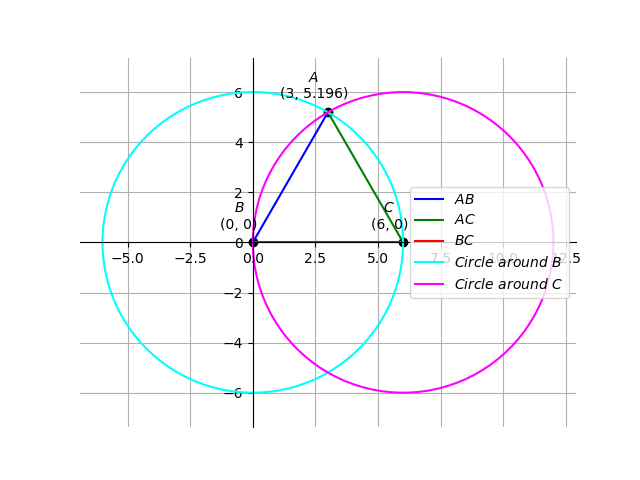
\includegraphics[width=10cm]{Figure_1.png}
\end{figure}









\end{document}
